\section{Durchführung}
\subsection{Übersicht}
Es finden insgesamt drei Versuchsteile statt. 
Im ersten Teil wird die Hysteresekurve eines Eisenkerns in einer Toroidspule bestimmt.
Beim zweiten Teil wird das Magnetfeld von einer kurzen und einer langen Spule in Abhängigkeit des Abstands untersucht.
Im letzten Teil werden für unterschiedliche Spulenabstände das Magnetfeld zwischen und hinter einem Spulenpaar in Abhängigkeit des Abstands ermittelt.
Hierfür werden zunächst alle nötigen Kenngrößen der einzelnen Spulen bestimmt bzw. mit den Angaben in der Anleitung \cite[]{man:v308} abgeglichen.
Radius und Länge der Spulen werden dabei mit einem Maßband gemessen,
Windungszahl und maximal zulässige Stromstärke werden den Beschriftungen der Spule und der Anleitung entnommen.
Des Weiteren stehen je nach Versuchsteil verschiedene Spannungstypen und Hallsonden zur Verfügung.
Vor jedem Versuch werden die Experimente im spannungslosen Zustand aufgebaut.
Beim Einschalten der Spannungsgeräte ist darauf zu achten, dass sowohl Strom $I$ als auch Spannung $U$ auf 0 geregelt sind.
Beim Einstellen ist auf die maximal zulässige Stromstärke zu achten.

\subsection[Hall-Sonde]{Die Hall-Sonde\footnote{Unter Verwendung der Quelle \cite{man:v308}.}}
Hall-Sonden sind Messgerät, die der Bestimmung der Magnetfeldstärke dienen.
Sie haben an ihrer Spitze ein Leiterplättchen, an dem ein Steuerstrom angelegt wird,
der senkrecht zum angelegten Magnetfeld verlaufen soll.
Dafür gibt es longitudinale und transversale Sonden, um je nach Situation messen zu können.
Allgemein gilt hierbei, dass das Leiterplätchen senkrecht zu den magnetischen Feldlinien orientiert sein soll.
Dementsprechend ist darauf zu achten, dass die Sonde möglichst senkrecht zum Feld orientiert ist.
Dadurch, dass Strom und Magnetfeld senkrecht auf einander stehen, wirkt eine Lorentzkraft auf die Ladungen.
Somit entsteht ein elektrischer Verschiebungsstrom.
Folglich wird eine Spannung, die sogenannte Hallspannung, aufgebaut.
Ist der angelegte Steuerstrom konstant, so ist die Hallspannung proportional zu Strom und magnetischer Flussdichte und
dadurch ein Maß für die Stärke des Magnetfeldes.
Dieser Effekt nennt sich auch Hall-Effekt.



\subsection{Hysteresekurve}
\label{sec:A_Hysterese_Drcf}
In dieser Versuchsreihe wird die Hysteresekurve mitsamt der Neukurve eines Eisenkerns in einer Toroidspule 
in Abhängigkeit der Stromstärke $I$ ermittelt.
Anhand der gemessenen Daten sollen Sättigungsmagnetisierung, Remanenz und Koerzitivkraft der Hysteresekurve bestimmt werden.
Außerdem sind differentielle Permeabilität für $H = 0$ und Sättigungswert der Neukurve zu ermitteln.

\noindent
Die Ringspule hat einen Luftspalt, damit an dieser Stelle eine transversale Hall-Sonde das Magnetfeld messen kann.
Der Anleitung wird eine Windungszahl von $n = 595$ und eine Breite des Luftspaltes von \qty[]{3}{\mm} entnommen.
Der Aufbau der Toroidspule ist weitestgehend vorbereitet, es muss nur das Spannungsgerät mit 2 Kabeln angeschlossen und die Hall-Sonde orientiert werden.
Da der Eisenkern noch eine gewisse Restmagnetisierung von vorherigen Versuchen haben kann,
wird zunächst eine Wechselspannungsquelle angeschlossen und ein starkes Wechselfeld eingestellt, um das Material zu entmagnetisieren.

\noindent
Im nächsten Schritt wird die eigentliche Spannungsquelle an die Spule angeschlossen.
Für eine Spannung $U = \qty[]{0}{\volt}$ und eine Stromstärke $I = \qty[]{0}{\ampere}$ wird der Wert der magnetischen Flussdichte abgelesen, 
die auch nach der Entmagnetisierung noch vorhanden ist.
Daraufhin wird die Stromstärke $I$ schrittweise um \qty[]{0.5}{\ampere} erhöht bis bei einem Wert von \qty[]{10}{\ampere} die Sättigung erreicht wird.
Dabei ist darauf zu achten, dass die Stromstärke nur in eine Richtung erhöht wird, um die Ergebnisse nicht zu verfälschen.
Falls also beim Erhöhen der Werte $I$ etwas zu groß eingestellt wird, darf es nicht niedriger geregelt werden.
Für jede eingestellte Stromstärke $I$ wird die magnetische Flussdichte $B$ in Abhängigkeit von $I$ notiert.
Mit Hilfe der hier gemessenen Daten können Neukurve sowie alle geforderten zugehörigen Größen ermittelt werden.

\noindent
Um die Kenngrößen der Hysteresekurve zu bestimmen, wird mit der gleichen Schrittweite $I$ stückweise bis zu \qty[]{0}{\ampere} gesenkt.
Anschließend wird umgepolt, wobei vor und nach dem Umpolen die magnetische Flussdichte für \qty[]{0}{\ampere} notiert wird.
Nach dem Umpolen wird erneut die Stromstärke bis \qty[]{10}{\ampere} erhöht und die eingestellten Werte von $I$ werden beim Notieren
mit einem negativen Vorzeichen versehen.
Anhand dieser Daten kann der obere Teil der Hysteresekurve bestimmt werden.
Der Vorgang wird wiederholt, damit auch der untere Teil der Kurve ermittelt werden kann.
Ein Foto des Versuchsaufbaus ist in Abbildung \ref{fig:hysterese_aufbau} zu sehen.


\begin{figure}[H]
    \centering
    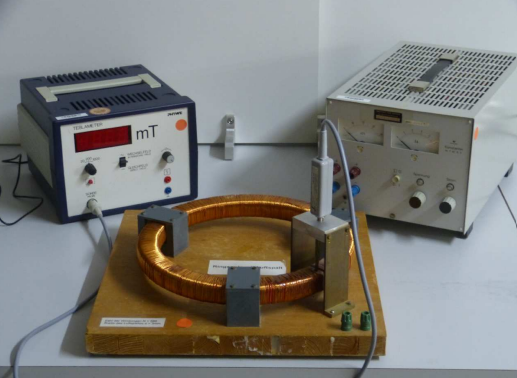
\includegraphics[height = 7cm]{abbildungen/toroidspule mit kern.png}
    \caption{Versuchsaufbau zur Bestimmung der Hysteresekurve \cite[]{man:v308}.}
    \label{fig:hysterese_aufbau}
\end{figure}

%Um die magnetische Flußdichte eines Toroides mit Eisenkern zu messen, muß ein Luftspalt eingefugt werden.


\subsection{Lange und kurze Spule}
Bei diesem Teil des Versuchs sollen die Magnetfelder $B$ von einer langen und einer kurzen Spule bei konstantem Strom in Abhängigkeit 
des Abstands $x$ ermittelt werden.
Die Werte für beide Spulen werden jeweils in einem $x$-$B$-Diagramm in Abschnitt \ref{sec:kurze_und_lange_Spule} dargestellt.
Es steht eine longitudinale Hall-Sonde zur Verfügung, die je nach Spule mittels eines Statives in der Höhe angepasst werden muss, 
sodass sie mittig von der Spule ist.
Das Leiterplättchen ist dabei auf der rechten Seite der Sonde.
Außerdem ist an dem Tisch eine Messlatte angeklebt, sodass die Abstände bestimmt werden können.
Für beide Messungen wird die Sonde bei der $\qty{50}{\cm}$ Marke des Lineals aufgestellt und die Spulen werden verschoben.
Das hat den Vorteil, dass die beiden gewählten Spulen jeweils auf bzw. in einem \enquote{Quader} montiert sind (vgl. abbildung \ref{fig:lange_kurze_spule}), 
die man längs des Lineals verschiebt,  sodass keine ungewollten Verschiebung in eine andere Richtung geschehen, wenn der eigentliche Abstand geändert wird.
Es müssen nur noch Spannungsgerät 

\noindent
Die Spulen werden so weit wie möglich über die Sonde geschoben und die Position des linken Randes wird abgelesen.
Um den Abstand von der Sonde zu der Spule besser darstellen zu können wird die $x$ Achse so gelegt, 
dass $x = 0$ ist, wenn die Sonde in der Mitte der Spule ist.

% Die Spule wird anschließend so weit wie es geht nach links über die Sonde gezogen und mit einem konstanten Strom betrieben.
% Die Position des linken Rands der Spule $x_\text{absolut}$ wird an der Messlatte abgelesen.
% Um den Abstand von der Sonde zu der Spule besser darstellen zu können wird die $x$ Achse so gelegt, 
% dass $x = 0$ ist, wenn die Sonde in der Mitte der Spule ist.
% Für die Transformation gilt also bei der langen Spule $x = x_\text{absolut} - \qty{50}{\cm} + \qty{8}{\cm}$ 

\begin{figure}
    \centering
    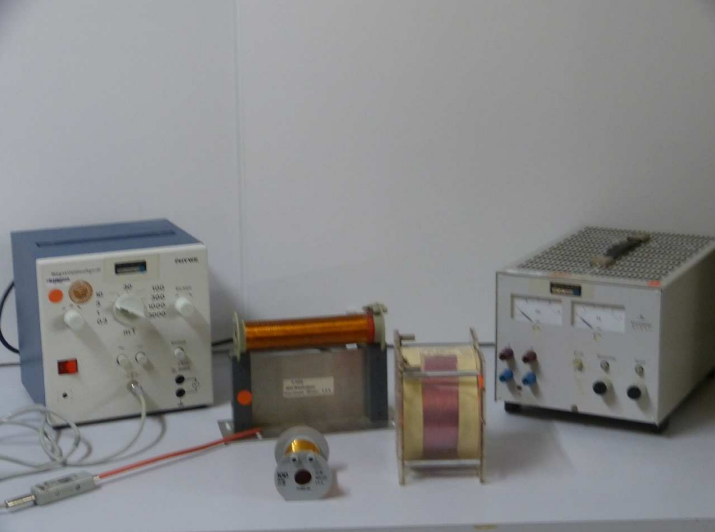
\includegraphics[]{abbildungen/lange und kurze spule.png}
    \caption[]{Versuchsaufbau zur Bestimmung der Magnetfelder einer langen und einer kurzen Spule \cite[]{man:v308}.}
    \label{fig:lange_kurze_spule}
\end{figure}

\subsubsection{Die kurze Spule}
Die kurze Spule hat die Windungszahl $n = 3400$, die Länge $l = \qty[]{9}{\cm}$, sowie einen Außendurchmesser von 
$D_\text{außen} = \qty[]{13}{\cm}$ und einen Innendurchmesser von $D_\text{innen} = \qty[]{8.5}{\cm}$.
Die Stromstärke $I$ beträgt \qty[]{0.6}{\ampere} und die Spannung $U = \qty[]{40}{\volt}$.


\subsubsection{Die lange Spule}

\subsection{Spulenpaar}
In diesem Versuchsteil wird das Magnetfeld eines Spulenpaars für unterschiedliche Spulenanstände in Abhängigkeit des Ortes der Sonde bestimmt.
Die beiden Spulen haben identische Parameter.
Hierfür wird der Anleitung \cite[]{man:v308} eine Windungszahl von $n = 100$, ein mittlerer Durchmesser von $D = \qty[]{125}{\mm}$ und eine 
Spulenbreite von $b = \qty[]{33}{\mm}$ entnommen.
Die beiden Spulen sind in Reihe geschaltet und haben dementsprechend eine identische Stromstärke $I$.
Um den Spulenabstand zu variieren, kann eine Spule verschoben werden, während die andere befestigt bleibt.
Es wird für die Spulenabstände \qty[]{24}{\cm}, \qty[]{12}{\cm} sowie \qty[]{6}{\cm} gemessen, wobei letzterer in etwa einer Helmholtz-Anordnung entspricht.
Je nach Spulenabstand werden unterschiedlich viele Messwerte zwischen und hinter dem Spulenpaar aufgenommen, wobei $x$ der Abstand vom 
rechten Rand der linken Spule zur Sonde in Abbildung \ref{fig:spulenpaar} ist.
Auch hier soll jeweils ein $x$-$B$-Diagramm für jeden Spulenabstand erstellt werden, vgl. Abschnitt \ref{sec:spulenpaar}.
Für die Messung des Magnetfeldes steht eine transversale Hall-Sonde zur Verfügung, die entlang einer oberhalb der Spulen montierten Schiene verschoben werden kann.
Auch hier muss auf die Orientierung der Sonde geachtet werden.
Sowohl an der Schiene als auch an der Befestigung für die Spulen ist jeweils ein Lineal, um den Abstand zwischen linker Spule und Sonde bzw. den Spulenabstand 
zu bestimmen.
Da die auf der linken Seite der Anordnung nicht richtig befestigt ist, wird sie festgehalten, um beim Verscheiben der Sonde Ungenauigkeiten zu reduzieren.



\begin{figure}[H]
    \centering
    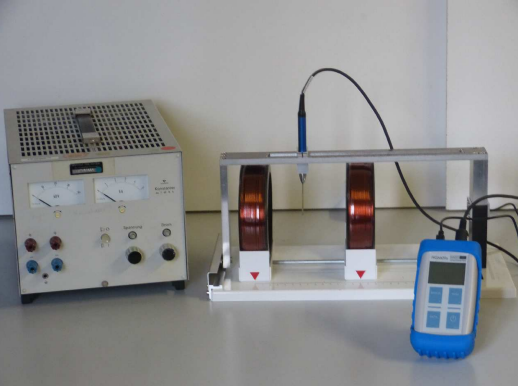
\includegraphics[height = 7cm]{abbildungen/spulenpaar.png}
    \caption{Versuchsaufbau zum Spulenpaar \cite[]{man:v308}.}
    \label{fig:spulenpaar}
\end{figure}


